\chapter{Implementation}
This chapter will describe the implementation of the entire system in the demonstrator.

\section{Platform}
To demonstrate the system, the RC car UTOR 8E from BSD racing was chosen. It has a steering servo, brushless DC motor, 

PWM signal to driver for motor and servo, 50Hz

\section{Electrical schematics}
Two 7.4V batteries in parallel. Voltage regulator to 5V for LIDAR, Raspberry Pi, encoders and WiFi module. Voltage regulator to DC input voltage for Zedboard.

\section{System overview}

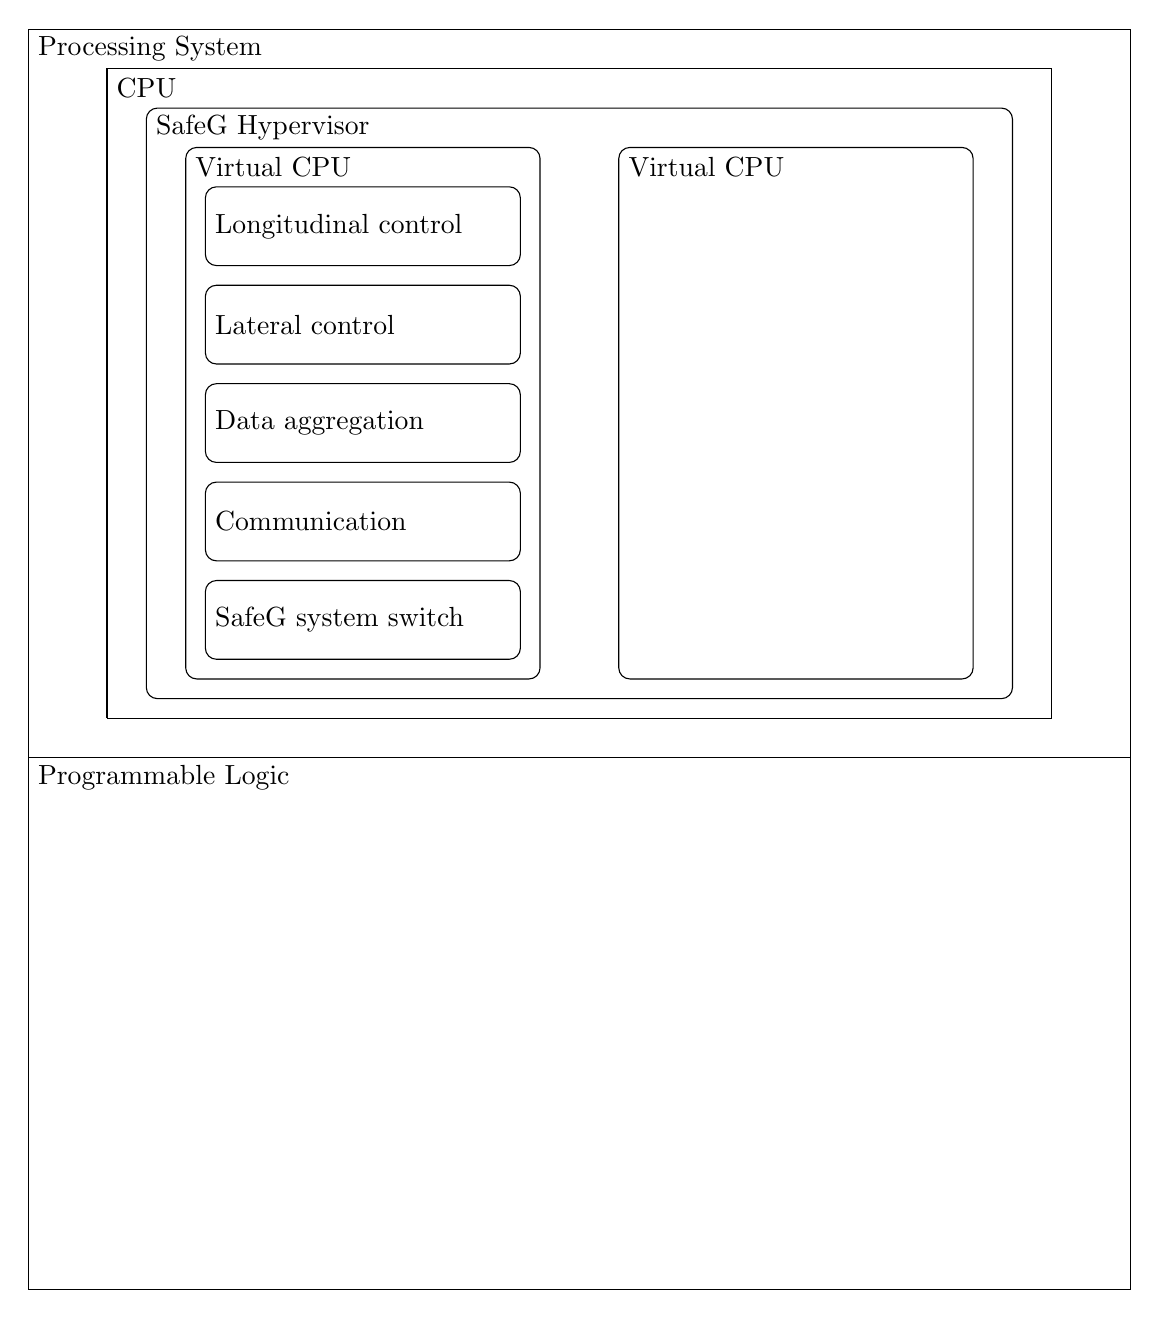
\begin{tikzpicture}

\draw (0,0) -- (14,0) -- (14,16) -- (0,16) -- (0,0);
\node [below, right] at (0,15.75) {Processing System};

\draw (1,7.25) -- (13,7.25) -- (13,15.5) -- (1,15.5) -- (1,7.25);
\node [below, right] at (1,15.25) {CPU};

\draw [rounded corners] (1.5,13) -- (1.5,7.5) -- (12.5,7.5) -- (12.5,15) -- (1.5,15) -- (1.5,13);
\node [below, right] at (1.5,14.75) {SafeG Hypervisor};

\draw [rounded corners] (2,13) -- (2,7.75) -- (6.5,7.75) -- (6.5,14.5) -- (2,14.5) -- (2,13);
\node [below, right] at (2,14.25) {Virtual CPU};

\draw [rounded corners] (7.5,13) -- (7.5,7.75) -- (12,7.75) -- (12,14.5) -- (7.5,14.5) -- (7.5,13);
\node [below, right] at (7.5,14.25) {Virtual CPU};

\draw [rounded corners] (2.25,13.5) -- (2.25,13) -- (6.25,13) -- (6.25,14) -- (2.25,14) -- (2.25,13.5);
\node [below, right] at (2.25,13.5) {Longitudinal control};

\draw [rounded corners] (2.25,12.5) -- (2.25,11.75) -- (6.25,11.75) -- (6.25,12.75) -- (2.25,12.75) -- (2.25,12.5);
\node [below, right] at (2.25,12.25) {Lateral control};

\draw [rounded corners] (2.25,11) -- (2.25,10.5) -- (6.25,10.5) -- (6.25,11.5) -- (2.25,11.5) -- (2.25,11);
\node [below, right] at (2.25,11) {Data aggregation};

\draw [rounded corners] (2.25,9.75) -- (2.25,9.25) -- (6.25,9.25) -- (6.25,10.25) -- (2.25,10.25) -- (2.25,9.75);
\node [below, right] at (2.25,9.75) {Communication};

\draw [rounded corners] (2.25,8.5) -- (2.25,8) -- (6.25,8) -- (6.25,9) -- (2.25,9) -- (2.25,8.5);
\node [below, right] at (2.25,8.5) {SafeG system switch};

\draw (0,6.75) -- (14,6.75);
\node [below, right] at (0,6.5) {Programmable Logic};

\end{tikzpicture}
